\documentclass{article}
\usepackage[utf8]{inputenc}
\usepackage{graphicx}

\title{Music Generation}
\date{December 2019}

\begin{document}

\maketitle

\section{Wave Lookup Synthesis}
In implementing the digital synthesis, we utilized a technique called Wavetable Lookup Synthesis, in
which a certain waveform is stored in a wavetable with constant access, and exploit the relation between
frequency and sampling rate to quickly build new waveforms. We used a single cycle (shown in Figure
1) sine wavetable as the basis for our additive and subtractive synthesis, sine wave is simplest of all waveforms and contains only a single frequency and no harmonics. All the other waveforms can be efficiently generated from sine by utilizing Fourier series of sine functions.  An example can be seen in Figure 2 where a sawtooth was generated. The sawtooth
waveform was then further used with subtractive synthesis to generate the pulse waveform shown in Figure 3. 

For each wave form we generate list of indexes, which we need to sample from the wave table. This indexes depend on frequency and harmonic and are not necessarily integers. To solve the complication caused by real indexes we use linear interpolation. 

For the implementation of wave table chose arrays over lazy-lists, despite the fact that list offer much more functionality, they are implemented as linked-lists, so does not give us access in constant time. 


Here comes figures

\section{Wave Forms}

There are four waveforms that are basis of any sound, these forms are sine wave, square wave, triangle wave and sawtooth wave. Besides these four, we also generate pulse and noise waves.
In our implementation we represent wave as Algebraic Data Structure ```:: Wave = Sine | Square | Triangle | Noise | Pulse | Sawtooth | Silence```. Our interface function, takes only 'Wave` type as parameter and generates respective wave as list of Real numbers.
For each wave form we need to define list of harmonics and list of amplitudes. In case of square, triangle and sawtooth this is simple, while for pulse and noise, more sophisticated technique had to be involved. 

\subsection{Sawtooth}
Frequency components are all harmonics, relative amplitudes are inverses of harmonic numbers and all harmonics are in phase.

% \begin{figure}[h!]
% 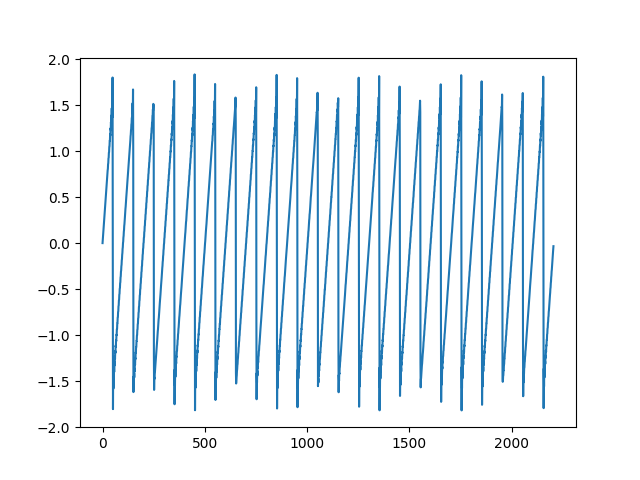
\includegraphics{saw.png}
% \label{fig:universe}
% \end{figure}

\begin{center}
    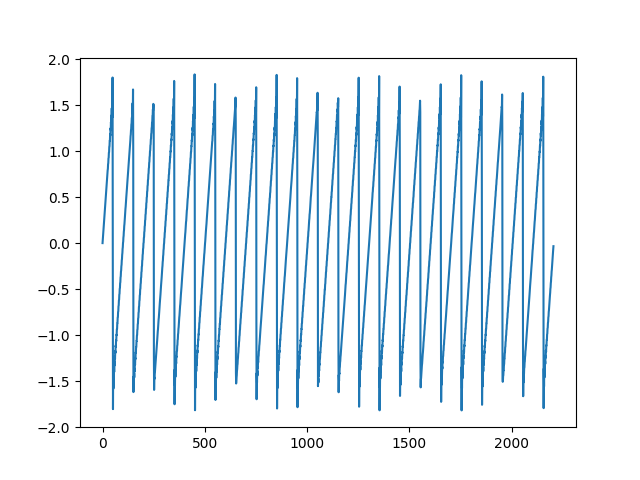
\includegraphics{saw.png}
\end{center}

\subsection{Square}
Frequency components are odd numbered harmonics, relative amplitudes are inverses of squares of harmonic numbers and all harmonics are in phase.

\begin{center}
    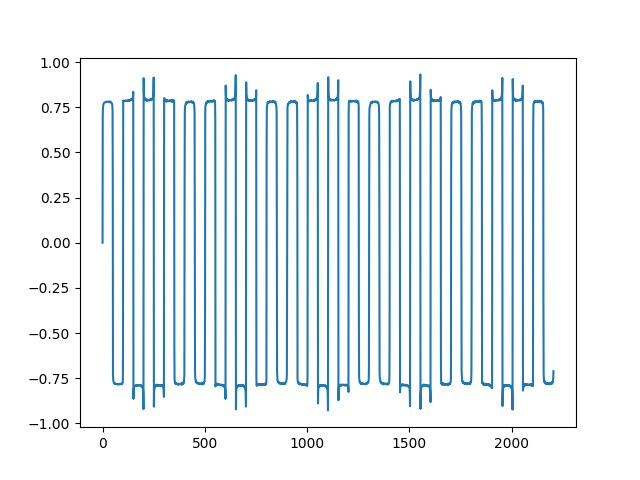
\includegraphics{square.png}
\end{center}


\subsection{Triangle}
Frequency components are odd numbered harmonics, relative amplitudes are inverses harmonic numbers and every second harmonic is 180 degrees out of phase. 

\begin{center}
    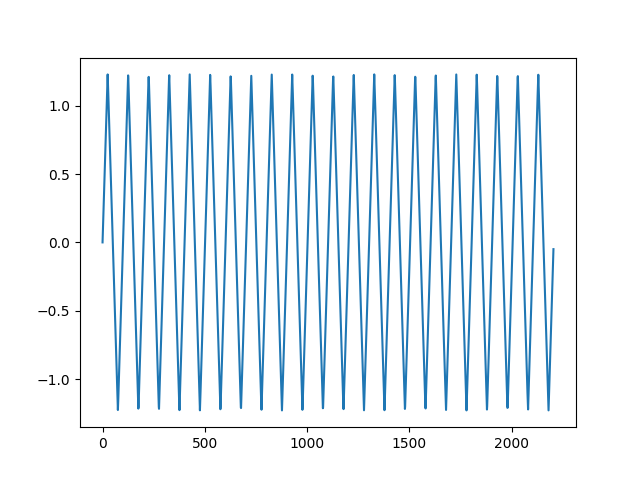
\includegraphics{triangle.png}
\end{center}


\subsection{Pulse}
To generate Pulse wave, we subtract Sawtooth wave from phase shifted version of itself. For this we have implemented efficient helper function `shiftLeft`, which moves every elemet of a list by given number to the left.  
\begin{center}
    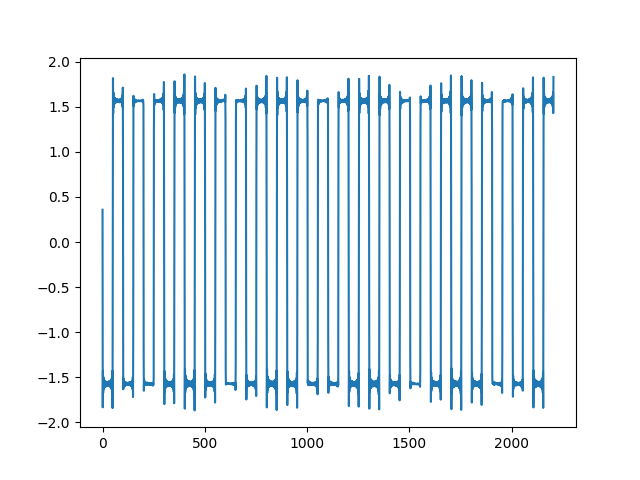
\includegraphics{pulse.png}
\end{center}


\subsection{Noise}
To generate Noise, we set all the amplitudes to 1 and harmonics to random numbers. Again we make use of our `shiftLeft` function, but this time we shift our lists by random number of places.
To generate random numbers, we use Clean built in module Math.Random, which provides pseudo random generator based on Mersenne Twister Algorithm.

\begin{center}
    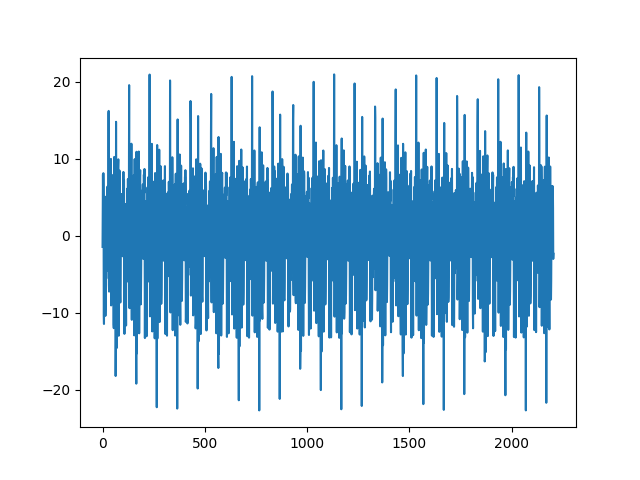
\includegraphics{noise.png}
\end{center}





\end{document}

